\section{Novel Contributions}\label{sec:novel-contributions}
This section deals with all those algorithms and methods that present a substantial element of novelty and that are at the core at the work carried out in this thesis.

\subsection{Algorithms} \label{subsec:algorithms-novel}
An important part of the work in this thesis was developing the algorithms needed to actually implement the ideas sketched in the paper \citep{Butz2018} (see Section \ref{sec:explaining-the-most-probable-explanation}).
The basic method was studied and adapted to the current case, including the construction of the \enquote{knowledge base} through a constructive dialogue with the domain expert and the generation of counterfactual explanation branches.
The current work goes beyond the ideas presented in the paper, as it aims to expand and validate these based on the wider explainability literature regarding Bayesian Networks (see Section \ref{sec:explainability-in-bayesian-networks}).
Thus the methods developed in this thesis aim to enable the actualisation of a mix of \textit{visual}, \textit{textual} and \textit{dialogical} interaction modes and support their subsequent validation in a real setting, by real medical domain experts.

\subsubsection{Dialogues} \label{subsubsec:dialogues}
The so-called \enquote{Pseudo-MPE} algorithm is inherently wrapped up with the concept of \textit{dialogue} and is central to the explanatory powers of the system being developed in this thesis.
The algorithm was developed as a way of implementing the \enquote{MPE branch} of the \enquote{Argumentative Probability Tree} hypothesised by \citet{Butz2018}.
It was termed \enquote{Pseudo-MPE} because it was noted that there are no guarantees of it returning the MPE solution and is confirmed by consulting \citep[pag. 26]{koller2007}.
The procedure proposed in the paper chooses the most probable (\enquote{strongest dependence}) item at each step and adds it to the \enquote{MPE probability tree} that is being built, as can be understood by looking at Figure \ref{fig:butz-tree} and \citep[sec. 3.1 and 4.3]{Butz2018}.
The procedure being advocated is equivalent to each variable in the data set \enquote{choosing} its most likely value in the current setting and is thus equivalent to:
\begin{quotation}
	\textit{[...]} the assignment where each variable individually picks its most likely value can be quite different from the most likely joint assignment to all variables simultaneously. This phenomenon can occur even in the simplest case, where we have no evidence.
	\hfill \citep[pag. 26]{koller2007}
\end{quotation}
An example showing how this may be the case is presented in Subsection \ref{subsec:bnupdating}.
This proves that the true MPE solution is not returned by such a procedure, thus the term \enquote{Pseudo-MPE}.

At a lower level of detail, the algorithm may be broken into:
\begin{itemize}
	\item a dialogical part, that interfaces with the expert user through the use of natural language, menus and visualisations
	\item the part responsible for constructing the \enquote{Pseudo-MPE branch}
\end{itemize}
The former process was informed and shaped by the results obtained by the methods described in Subsection \ref{subsec:explainability-validation}.

The latter part is, at its core, a greedy procedure that aims to select the \enquote{best} next \textit{(state,value)} tuple at each step, based on some measure of optimality and on the variables already in the evidence set.
In the actual implemented system the two parts are intertwined, given their close inter-dependence.

The \texttt{dialogue} procedure starts by asking the user to select a subset of variables and their relative values to add as initial evidence.
This initial evidence is used to radicate the MPE Branch.
It should be noted than in the description given by \citet{Butz2018}, the Argumentative Probability Tree is a real tree (Definition \ref{def:tree}) as each node is guaranteed to have at most one parent.
This application, on the other hand, constructs an \textit{Argumentative Probability Polytree} (Definition \ref{def:polytree}) because, as will better be described in Chapter \ref{chap:results}, it was seen early on that the users much preferred to be able to start from a set of initial evidences and not be limited to a single one.

The algorithm then proceeds to call the \texttt{next\_most\_probable\_states} subroutine that is tasked with returning an ordered list of \textit{(state,value)} pairs.
It does this by calculating the posterior distribution given evidence of all the states not already in the evidence, then calculating the efficiency (Definition \ref{def:mutual-information} ) and the maximally probable symbol of each state's distribution and finally returning the \textit{(state,value)} tuples ordered according to the normalised entropy of the states (see Subsection \ref{subsec:entropy}).
The least entropic states is thus at the head of the list.

The \textit{(state,value)} pair at the head of the list is proposed to the user who has the faculty to accept the system's proposal or refuse it.
If the user accepts it, the proposed tuple is added to the evidence set and to the Pseudo-MPE Branch under construction.
Thus, the evidence set's cardinality increases by one each time a user accepts a proposal.
The updated evidence will be used to calculate the new list of \textit{(state,value)} pairs at the following round.

If the expert chooses to refuse, then she is iteratively presented with the remaining \textit{(state,value)} items, in order of decreasing efficiency. 
This is explained, and justified, in detail in Subsection \ref{subsec:entropy-based-selection}.
Once she accepts one of the explanations given by the system, the \texttt{generate\_alternative\_branch} subroutine is called to automatically generate a maximally probable Pseudo-MPE Branch, radicated in the newest \textit{(state,value)} node of the MPE Branch (the algorithm is described in Subsection \ref{subsec:algorithms-novel} under the \textbf{Alternative Explanation Branches} header).

The proposal loop for alternative states runs until there are increasingly less probable elements in the list and exits with a partial solution if the user refuses all of them at a given step.

Three slightly different operational modes of the algorithm were implemented.
This was done for research purposes, in order to understand which of the three, if any, the expert users would find the best from a usability, comprensibility and explainability standpoint
In alternative, the question was to understand if a combination of their distinctive features were preferred over any single one.
\begin{itemize}
  \item \textit{exhaustive}: in the basic dialogue mode, the set of variables under consideration monotonically decreases by one every time the user accepts a system's proposal and the dialogue terminates only when the user has accepted all variables at least once or refused all proposals at a given step.
	In the first case the user will have the Pseudo-MPE solution while in the second she will be left with a partial assignment to some of the variables not present in the initial evidence.
	The pseudocode is shown in Algorithm \ref{alg:pseudo-mpe-exhaustive}.
  \item \textit{d-separated}: in the second variant, the set of variables considered at each step is dynamic and depends on the separation properties of the underlying Bayesian Network's DAG and on the evidence set constructed by the user's choices.
  
  	Differently from the first type of dialogue, an additional \texttt{evidence\_d\_separation} subroutine is called before \texttt{next\_most\_probable\_states} to calculate the set of variables that are d-separated from the evidence set, up to that step of the dialogue.
  	\texttt{next\_most\_probable\_states} is then executed but the variables that the previous function found to be separated from the evidence, are removed from the returned list.
  	This way, variables that can have no effect given the current evidence are not proposed.
  	
  	As the d-separation operation is not monotonic, adding new nodes to the evidence set can both increment or diminish the number of nodes that will be proposed at each step.
  	D-separation is not \enquote{monotonic} because, as can be understood by looking at the definitions of when a v-structure is \textit{closed} given in Subsection \ref{subsec:d-separation}, a \textit{collider} is only closed when its central node is \textit{not} in the evidence set.
  	Thus, if a new node is added to evidence it is liable to \textit{open} some v-structure and thus may make previous d-separated nodes become d-connected.
  	
  	The user is shown an updated view of the independencies of the graph at each step; an example of such an output is shown in Figures \ref{fig:pseudo-mpe-independencies_1} and \ref{fig:pseudo-mpe-independencies_2}.
  	The pseudocode is shown in Algorithm \ref{alg:pseudo-mpe-independencies}.
  \item \textit{thresholded}: the final variant of the algorithm, prunes the set of variables using a different strategy from the previously presented one.
  	In this case, the \textit{(state,value)} pairs in the list returned by \texttt{next\_most\_probable\_states} are dropped automatically based on their probability.
  	Pairs whose probability is below a user-defined threshold or are \enquote{worse than random} (for ex. a \textit{(state,value)} tuple will be discarded if $state$ is binary and the probability of $value$ is lower than $0.5$) are removed and not proposed to the user. 
  	
  	This thresholding strategy based on the probability of the tuples is paired with a threshold on the number of times that the expert can refuse a particular \textit{(state,value)}. 
  	
  	In the general dialogue, tuples can be proposed multiple times, with an ever lower probability, if the user has previously refused them; in the thresholded scheme a \textit{(state,value)} pair can only be proposed a maximum number of times before being permanently discarded.
\end{itemize}

The underlying Bayesian Network representing the data set is learned and queried through the  \texttt{Pomegranate} (see Subsection \ref{subsec:libraries}), API but the great majority of all the code is completely custom-written.
This was necessary because \texttt{Pomegranate}, while having a powerful backend, was found to be severely lacking in the breadth and flexibility of its API.
Many basic operations, such as the calculation of a joint distribution, were not available so the only way was to implement lower-level workarounds while still using \texttt{Pomegranate} for the most basic operations, for example the calculation of a posterior distribution.
In particular, \texttt{dialogue} is implemented with the only direct calls to the API being when learning the network and when calling \texttt{predict\_proba}, that queries the \texttt{BayesianNetwork} object to calculate the posterior distribution of the states given the current evidence.
D-separation, in the second variant of the algorithm, is calculated via the \texttt{evidence\_d\_separation} procedure that implements the pseudocode presented in Algorithm \ref{alg:d-separation}.

\subsubsection{Alternative Explanation Branches}
The function to generate alternative branches to the main Pseudo-MPE branch in the dialogue tree is called after the user refuses a \textit{(state,value)} in the dialogue and accepts one of the the alternatives.

The motivation for this functionality is to present the user with a \enquote{what-if} analysis, thus helping in replying to the question \enquote{had I accepted the \textit{(state,value)} presented me by the system, what would have been the most probable configuration of the remaining \textit{(state,value)} pairs?}.
The question is answered by generating a maximally probable, alternative Pseudo-MPE sub-branch that rooted in the last node in the main Pseudo-MPE branch.

The alternative branch is generated by what is essentially an automated version of \texttt{dialogue}, that always accepts the first suggestion returned by \texttt{next\_most\_probable\_states}, compatibly with the pruning strategy of the main \texttt{dialogue}.
Given that \texttt{dialogue} and \texttt{generate\_alternative\_branch} are essentially one and the same, the latter inherits the same pruning strategies as the former.
That is, \texttt{generate\_alternative\_branch} called during the exhaustive dialogue will generate a maximally likely assignment over all variables in $V \smallsetminus E$ while when invoked from one of the other two variant of the dialogue algorithm, it will apply their same pruning strategies.

The implementation of the Pseudo-MPE Polytree is based on the NetworkX Python package (see the relative header in Subsection \ref{subsec:libraries}).
The creation of a chain of nodes is done by keeping a local pointer $alt\_node$ that refers to the last added node or set of nodes, if the node being added is the successor of multiple initial evidences. 

An example of the output shown to the user at each step of the dialogue is shown in Figure \ref{fig:alternative-branch} while the pseudocodes for the three variants are shown in Algorithms \ref{alg:alternative-branch-exhaustive}, \ref{alg:alternative-branch-independencies} and \ref{alg:alternative-branch-thresholded}.
Note that $alternative\_evidence$ is local to this algorithm and is separate from the $evidence$ used in the main \texttt{dialogue} procedure.

\subsubsection{\enquote{Pseudo-MPE} from Initial Evidence} \label{subsubsec:pseudo-mpe}
In order to compare the Pseudo-MPE output with the true MPE solution, an algorithm was implemented that, starting from an initial set of evidence, generated the relative pseudo-MPE solution.
The random initial evidence set is constructed by stochastically choosing a number in the interval $k = [ 1, |V| ]$, with $V$ the set of vertices in the BN, and then randomly selecting $k$ of the random variables in $V$ to yield the set of variables $E$.
The value of each variable is randomly chosen among the set of its values; as all variables are categorical and thus discrete, this is straightforward.

An optional threshold can be set by the user in order to discard \textit{(state,value)} pairs whose probability is deemed too low.

The implementation is based on the NetworkX Python library (see Subsection \ref{subsec:libraries} under the relative header) package as what is being constructed is not a tree but a \textit{polytree} (Definition \ref{def:polytree}), as nodes may have multiple parents.
Note that $alternative\_evidence$ is considered separate from the main $evidence$ used in \texttt{dialogue}.
The pseudocode is shown in Algorithm \ref{alg:pseudo-mpe-initial-evidence}.

\subsubsection{MPE Algorithms Comparison}
In order to compare the quality of the solution found using the simple Pseudo-MPE heuristic, an experiment was set up to compare it to the exact MPE solutions.

The user is asked to select the number of iterations over which to average the results and at each one of these a Pseudo-MPE solution is generated using Algorithm \ref{alg:pseudo-mpe-initial-evidence}.
The same initial evidence is fed to DAOOPT using the \texttt{daoopt\_solver} interfacing procedure shown in Subsection \ref{subsec:algorithms} and to Pgmpy's \texttt{map\_query} function.

At each iteration corresponds a random evidence; the solutions given by the Pseudo-MPE, Pgmpy and by DAOOPT are scored against each other using Hamming (Definition \ref{def:hamming}) and Jaccard (Definition \ref{def:jaccard}) distances on the vectors representing the returned assignments.
The sequence of distances is then averaged over all the iterations to return the averaged distances between the three solutions to the MPE problem.

The implementation of the algorithm had to deal with the fact that DAOOPT failed on certain configurations of input evidence.
The reason for this is unknown so the workaround was to discard any iterations where DAOOPT had failed and retry them with another random set of evidences.

\subsubsection{Pairwise Correlations} \todo[inline]{come giustifico che sia `novel'?}
An interesting addition, in terms of both explainability and as a \textit{novel contribution}, is the implementation of an algorithm to measure and graphically display the interrelatedness between pairs of variables.
The Definition \ref{def:mutual-information} of mutual information presented is extended to account for the current state of the model i.e., the set of observed variables.
To the best of our knowledge, there has been no work that has applied this method to Bayesian Networks.

The \textit{conditional mutual information} between each pair of parent $\rightarrow$ child variables is calculated as:
\begin{equation}
	I(X,Y|\boldsymbol{E}=\boldsymbol{e}) = \sum\limits_{x \in \mathcal{X}} \sum\limits_{y \in \mathcal{Y}} \mathbb{P}(X=x,Y=y \mid \boldsymbol{E}=\boldsymbol{e}) \log_{b} \left( \frac{\mathbb{P}(X=x,Y=y \mid \boldsymbol{E}=\boldsymbol{e})}{\mathbb{P}(X=x \mid \boldsymbol{E}=\boldsymbol{e}) \mathbb{P}(Y=y \mid \boldsymbol{E}=\boldsymbol{e})} \right)
\end{equation}
This is not done if the parent or child variable, in the $X \rightarrow Y$ tuple under consideration, is in the evidence set; this because observing a variable in a BN conceptually corresponds to disconnecting it from its children.

The implementation takes advantage of Pgmpy's \citep{pgmpy} inference capabilities. 
To do this, a function to convert a Pomegranate-based BN to an equivalent Pgmpy-based one had to be written.
The queries to the model are then done using the variable elimination algorithm, that is more than suitable for a small BN like the one built upon the provided data set (described in Section \ref{sec:data-set}).
The marginals $\mathbb{P}(X)$ $\mathbb{P}(Y)$ for $X$ and $Y$ are calculated directly from the joint distribution $\mathbb{P}(X,Y)$, by marginalising it over one variable and then with respect to the other.

The function exits with $-1$ if the parent or child variable is in the evidence set.
As mutual information $I(X,Y) \in [0,1]$, this signals to the calling function to treat this pair of variables differently.
The pseudocode for the algorithm is shown in Algorithm \ref{alg:mutual-information}.

\subsection{Interfacing with the User} \label{subsec:interfacing-user}
The driving design \textit{desideratum} was for the system to be as transparent to the final user as possible.
This intent was shared by the Istituto Cantonale di Patologia, whose members felt strongly about not wanting to have to deal with the inner workings and algorithms of the system but be able to only concentrate on the data and task at hand.

The interactions with the system were designed to take advantage of the best practices identified in the literature review in Section \ref{sec:explainability-in-bayesian-networks}.
Thus, natural language was identified as the most spontaneous way to make the expert user aware of the knowledge in the data set and for her to interact with the system, given that \citet{lacave2002review} identify verbalisation as the most naturally comprehensible output format for humans.
Thus the main interaction mode with the implemented system is in using natural language, both as input and as output.
Natural language denominators come \enquote{for free} when dealing with the node names and their values, regardless of their internal representation in the implemented model, as these are simply the column names and values found in the original input data set.
A bit more care needs to be taken when quantifying probabilities to the user; these should be \enquote{linguistic probabilities} as suggested by \citet{henrion1990qualtitative}.
The format chosen should fit in as seamlessly as possible with the rest of the phrases generated and be able to conform to the user's preconceptions regarding probabilities.
It should be both \textit{informative} and \textit{precise}.
The chosen coding was taken from \citet{Butz2018} and is shown in Table \ref{tab:naturallanguageprobabilities}.
The mapping is used every time there is a need to translate a probability into natural language to be output to the user; for example when proposing tuples during a Dialogue (see Subsection \ref{subsubsec:pseudo-mpe}) as example of which can be seen in Figure \ref{fig:nl-dialogue}.

In Figures \ref{fig:nl-independencies}, \ref{fig:nl-conditional} and \ref{fig:nl-mpe} we can see how the interface to the system's functions leans heavily on natural language elements.
The design ideal was for the system to be as accessible and the least intimidating possibile, so that the user may be able to extract the maximum amount of information in an easy way.
Not only the terms but also the phrasing were deemed to be important: every interaction is broken down into what are though to be manageable steps.
For example, a user isn't asked to provide all evidences at once but is asked for one at a time, when necessary.
The idea is to reduce cognitive overload on the expert's part so that he may be able to better concentrate on the task at hand, not on the tool he is using to achieve it.

Another important aspect is to translate the information into a language that would make semantic sense to the user; that is it should be part of the user's \textit{ontology}, the set of concepts part of his World.
This can be seen in Figure \ref{fig:nl-independencies} where the notion of d-separation in the underlying BN's DAG is remapped to a higher-level concept that is part of the user's ontology, like that of variables affecting each other's values or not.
The underlying theme of the work carried out in this thesis is to translate \textit{information} present in a data set into \textit{knowledge} for a medical expert user.
This is done in various ways, for example through the use of dialogue, in order to bring the data to a form that is manageable and comprehensible.

\citet{lacave2002review} identify that \enquote{the most direct and intuitive way of showing the information embodied in a Bayesian network is to display the corresponding graph}.
For this reason, visualisations are used extensively throughout all interactions modes, as can be seen from the multitude of figures through this chapter. 

A final element is that of a coherent use of colours, even in the experimental command-line interface that has currently been developed.
This may seem secondary, but many of the BN-based systems surveyed by \citet{lacave2002review} took extensive advantage of colours in their visualisations.
In the generated phrases the source variables are always highlighted in \textit{magenta}, the evidences in \textit{green} and the results of the queries in \textit{cyan}.
It is hoped that this guide the user's eye towards the important elements of what he had set out to achieve, thus anchoring her experience and letting the marginal elements fade into background.

The grammars for the generation of the natural language are presented in Algorithms \ref{alg:nl-dialogue}, \ref{alg:nl-independencies}, \ref{alg:nl-conditional} and \ref{alg:nl-mpe}; these are defined in Extended Backus-Naur form (EBNF).

One of the most important parts of this work is the validation of this interface with real medical expert users, the results of which are presented in Chapter \ref{chap:results}.
This is done in order to address one of the main gaps identified in the current literature: the lack of \textit{application-grounded evaluations} (see Section \ref{sec:evaluation-of-explainability}).

\subsection{Entropy-Based Selection} \label{subsec:entropy-based-selection}
The criterion for the selection of the strongest dependencies while constructing the \enquote{knowledge base}, as defined by \citet{Butz2018} and described in Section \ref{sec:explaining-the-most-probable-explanation}, is not the probability but the \textit{normalised entropy} of each item.
In the case of the methods currently under examination, such items are \textit{(state,value)} pairs with the \textit{value} being the most probable among the categorical \textit{state}'s values.
For example, the tuple for the state shown in Figure \ref{fig:entropy-example-1} would be \textit{(X, b)}.
Among all available \textit{(state,value)} pairs, the one whose \textit{state} has lowest normalised entropy is chosen as the strongest dependency to be added to the \enquote{knowledge base}.

If states are of the same cardinality, then the one selected will be the one presenting a value with a probability higher than that of all other states in the other variables.
Within each state, the most probable value (the one with highest probability) is the one chosen to be paired in the tuple \textit{(state,value)}.
The state selected will be the least entropic i.e., the one whose KL divergence (Definition \ref{def:kl-divergence}) from the uniform distribution is greatest; this state will necessarily be the one with the highest \enquote{probability peak} on one of its values.
Thus, in the case where variables have the same cardinality, selecting the most probable \textit{(state,value)} pair based on the \textit{value}s' probabilities or on the normalised entropy of the state gives the same result.
Using normalised entropy as the state selection criterion, thus factoring out the variable cardinality, makes this result applicable to states with a dishomogeneous number of values.
\todo[inline]{va bene?  modi migliori di giustificare la cosa, tirando magari in ballo anche information gain?}

This normalised entropy-based selection method, that a review of the literature hasn't surfaced as having been used either within or outside the xAI community, is justified by the intuition that simply selecting based on the probability of the values results in a bias against higher cardinality variables.
Assuming that the underlying process generating the variables is similar, for example Gaussian, then a variable with higher cardinality will see its probability mass more spread out i.e., it will be less \enquote{dense}.
An example of this phenomenon can be seen by comparing the distribution of the variable displayed in Figure \ref{fig:entropy-example-2} with that of Figure \ref{fig:entropy-example-1}.

\begin{figure}[htbp]
\centerline{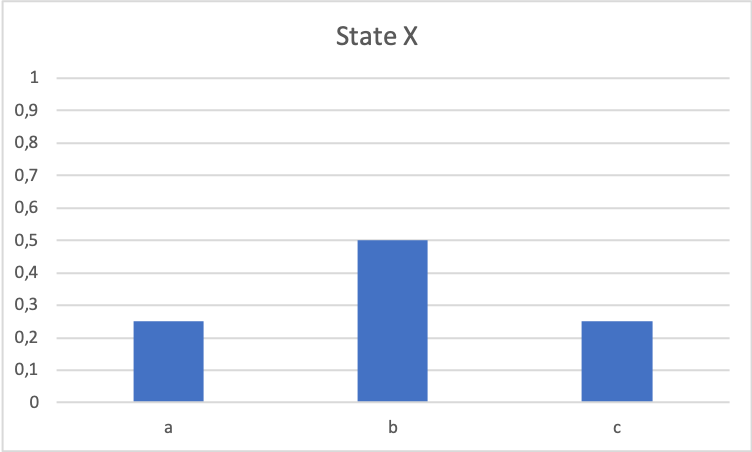
\includegraphics[width=0.5\textwidth]{methodology/images/entropy-example-1}}
\caption{Distribution of state $X$ with possible values \textit{a}, \textit{b} and \textit{c}}
\label{fig:entropy-example-1}
\end{figure}

\begin{figure}[htbp]
\centerline{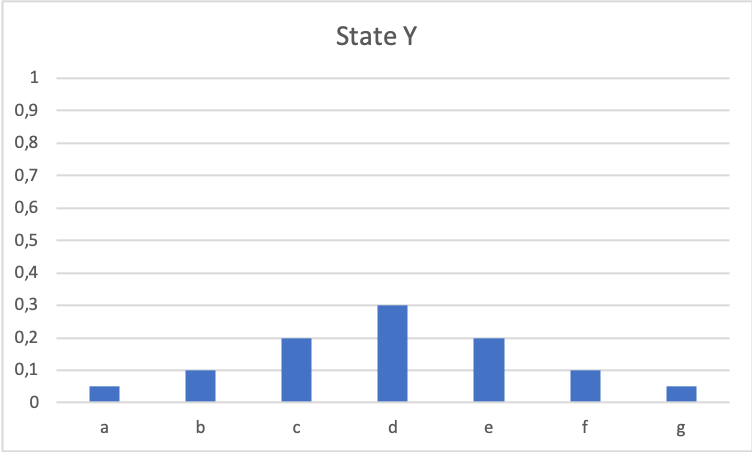
\includegraphics[width=0.5\textwidth]{methodology/images/entropy-example-2}}
\caption{Distribution of state $Y$ with possible values \textit{a}, \textit{b} and \textit{c}}
\label{fig:entropy-example-2}
\end{figure}

\begin{algorithm}[htp!]
	\caption{Exhaustive dialogue algorithm}
	\label{alg:pseudo-mpe-exhaustive}
	\begin{algorithmic}[1]
		\State $evidence = $ user selected \textit{(state,value)} tuples
		\State $MPE\_polytree = $ MPE Polytree rooted in $evidence$
		\While{True} 
			\State $mpe\_states$ = \texttt{next\_most\_probable\_states($evidence$)}
			\If{$mpe\_states$ is not empty}
				\State $next\_state$ = head of $mpe\_states$ 
				\State propose $next\_state$ to user \Comment{the least entropic state}
				\If{the user refuses $next\_state$}
					\For{$alternative\_state$ in $mpe\_states \smallsetminus next\_state$}
						\State propose $alternative\_state$ to user \Comment{the next least entropic states}
						\If{the user accepts $alternative\_state$}
							\State call \texttt{generate\_alternative\_branch()} on $MPE\_polytree$ 
							\State add $alternative\_state$ to $MPE\_polytree$
							\State $evidence = evidence \cup alternative\_state$
						\Else
							\State continue
						\EndIf
					\EndFor
				\Else
					\State add $next\_state$ to $MPE\_polytree$
					\State $evidence = evidence \cup next\_state$
				\EndIf
			\Else 
				\State return
			\EndIf
		\EndWhile
	\end{algorithmic}
\end{algorithm} 

\begin{algorithm}[htp!]
	\caption{Independencies dialogue algorithm}
	\label{alg:pseudo-mpe-independencies}
	\begin{algorithmic}[1]
		\State $evidence = $ user selected \textit{(state,value)} tuples
		\State $MPE\_polytree = $ MPE Polytree rooted in $evidence$
		\While{True} 
			\State $separated = $ \texttt{evidence\_d\_separation($evidence$)} \Comment{based on evidence of previous step}
			\State $mpe\_states$ = \texttt{next\_most\_probable\_states($evidence$)}
			\State $mpe\_states = mpe\_states \smallsetminus separated$ 
			\If{$mpe\_states$ is not empty}
				\State $next\_state$ = head of $mpe\_states$ 
				\State propose $next\_state$ to user \Comment{the least entropic state}
				\If{the user refuses $next\_state$}
					\For{$alternative\_state$ in $mpe\_states \smallsetminus next\_state$}
						\State propose $alternative\_state$ to user \Comment{the next least entropic states}
						\If{the user accepts $alternative\_state$}
							\State call \texttt{generate\_alternative\_branch()} on $MPE\_polytree$ 
							\State add $alternative\_state$ to $MPE\_polytree$
							\State $evidence = evidence \cup alternative\_state$
						\Else
							\State continue \Comment{go to next proposal}
						\EndIf
					\EndFor
				\Else
					\State add $next\_state$ to $MPE\_polytree$
					\State $evidence = evidence \cup next\_state$
				\EndIf
			\Else 
				\State return 
			\EndIf
		\EndWhile
	\end{algorithmic}
\end{algorithm} 

\begin{figure}[htbp]
\centerline{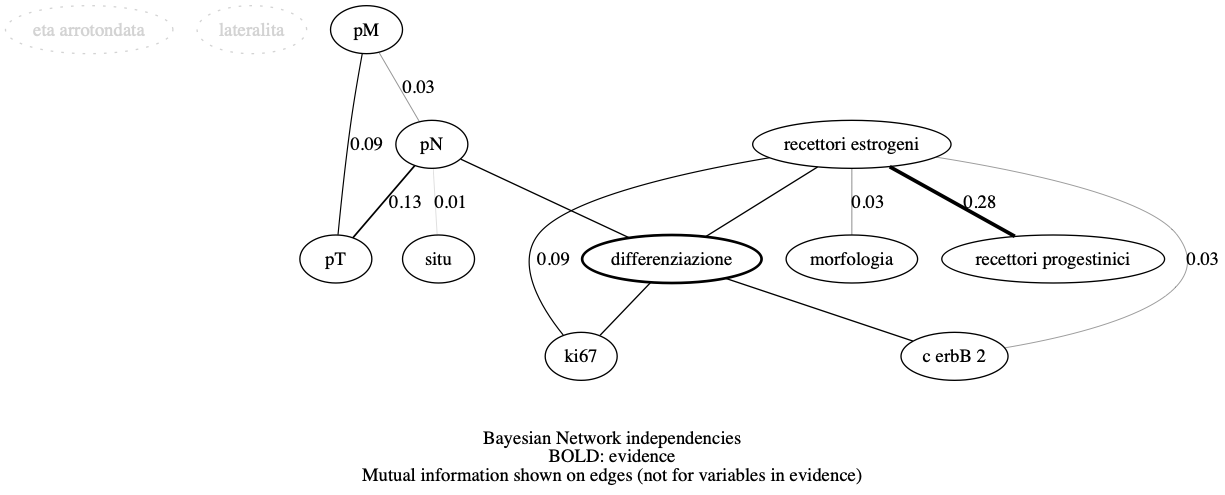
\includegraphics[width=\textwidth]{methodology/images/example-d-separation-mpe_1}}
\caption{Example output during the first round of the d-separation-aware variant of \texttt{dialogue}.
	The variable \enquote{differenziazione} is the initial evidence.}
\label{fig:pseudo-mpe-independencies_1}
\end{figure}

\begin{figure}[htbp]
\centerline{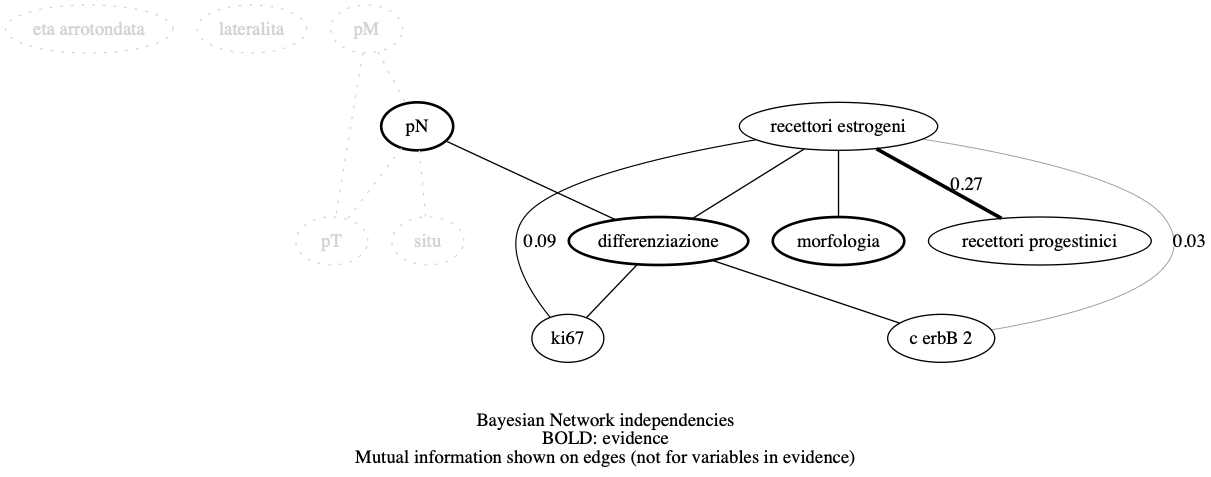
\includegraphics[width=\textwidth]{methodology/images/example-d-separation-mpe_2}}
\caption{Example output during the third round of the d-separation-aware variant of \texttt{dialogue}.
	\enquote{pN} and \enquote{morfologia} are added to the evidence set and this makes a part of the network redundant.}
\label{fig:pseudo-mpe-independencies_2}
\end{figure}

\begin{algorithm}[htp!]
	\caption{Thresholded dialogue algorithm}
	\label{alg:pseudo-mpe-thresholded}
	\begin{algorithmic}[1]
		\State user selected $refuse\_bound$
		\State $refuse\_thresholds = \emptyset$
		\State $lower\_thresholds = \emptyset$
		\For{$v \in V$}
			\For{value $k$ of $v$}
				\State element $[v,k]=0$ in $refuse\_thresholds$
			\EndFor
			\State element $[v]=1 / |v|$ in $lower\_thresholds$ \Comment{refuse worse than random pairs}
		\EndFor
		\State $evidence = $ user selected \textit{(state,value)} tuples
		\State $MPE\_polytree = $ MPE Polytree rooted in $evidence$
		\State $mpe\_states$ = \texttt{next\_most\_probable\_states($evidence$)}
		\While{True} 
			\For{$s \in mpe\_states$}
				\If{probability of $s < lower\_thresholds[s] \wedge refuse\_thresholds[s] > refuse\_bound$}
					\State remove $s$ from $mpe\_states$ 
				\EndIf
			\EndFor		
			\If{$mpe\_states$ is not empty}
				\State $next\_state$ = head of $mpe\_states$ 
				\State propose $next\_state$ to user \Comment{the least entropic state}
				\If{the user refuses $next\_state$}
					\State increment $refuse\_thresholds[next\_state]$
					\For{$alternative\_state$ in $mpe\_states \smallsetminus next\_state$}
						\State propose $alternative\_state$ to user \Comment{the next least entropic states}
						\If{the user accepts $alternative\_state$}
							\State call \texttt{generate\_alternative\_branch()} on $MPE\_polytree$ 
							\State add $alternative\_state$ to $MPE\_polytree$
							\State $evidence = evidence \cup alternative\_state$
						\Else
							\State increment $refuse\_thresholds[alternative\_state]$
							\State continue
						\EndIf
					\EndFor
				\Else
					\State add $next\_state$ to $MPE\_polytree$
					\State $evidence = evidence \cup next\_state$
				\EndIf
			\Else 
				\State return
			\EndIf
		\EndWhile
	\end{algorithmic}
\end{algorithm} 

\begin{figure}[htbp]
\centerline{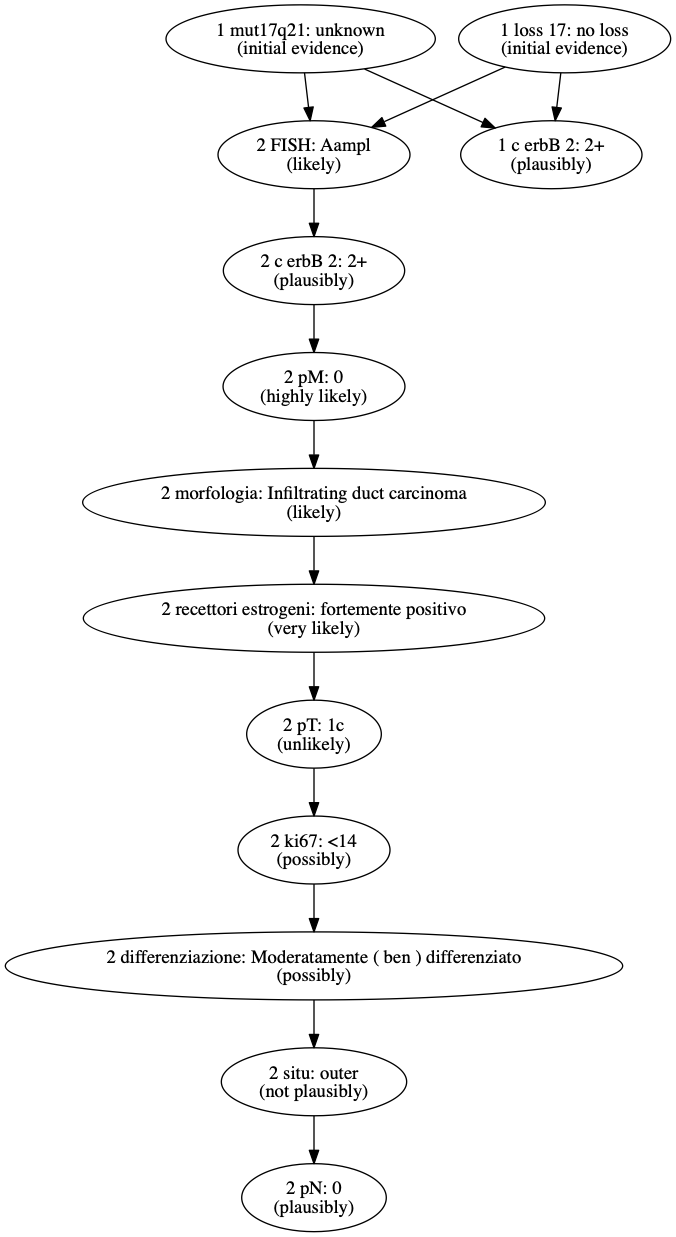
\includegraphics[scale=0.2]{methodology/images/alternative-explanation-tree-example}}
\caption{Example output during the d-separation-aware variant of \texttt{dialogue}.
	The tuple (\enquote{FISH},\enquote{Aampl}) was proposed but the expert refused it and accepted the alternative (\enquote{c erbB 2},\enquote{2+}).
	The main Pseudo-MPE Branch has ID 1 while the \enquote{what-if} one has ID 2.}
\label{fig:alternative-branch}
\end{figure}

\begin{algorithm}[htp!]
	\caption{Exhaustive alternative explanation branch algorithm}
	\label{alg:alternative-branch-exhaustive}
	\begin{algorithmic}[1]
		\State $alternative\_evidence = evidence$ 
		\State $alt\_node = $ last node in the main MPE Polytree
		\State $branch\_id = branch\_id + 1$
		\While{True} 
			\State $mpe\_states$ = \texttt{next\_most\_probable\_states($alternative\_evidence$)}
			\If{$mpe\_states$ is empty}
				\State return
			\Else
				\State $next\_state$ = head of $mpe\_states$ 
				\State create $next\_state$ node, tag it with $branch\_id$ and make it son of $alt\_node$
				\State update $alt\_node$ node to be $next\_state$ node
				\State $alternative\_evidence = alternative\_evidence \cup next\_state$
			\EndIf
		\EndWhile
	\end{algorithmic}
\end{algorithm}

\begin{algorithm}[htp!]
	\caption{Independencies alternative explanation branch algorithm}
	\label{alg:alternative-branch-independencies}
	\begin{algorithmic}[1]
		\State $alternative\_evidence = evidence$ 
		\State $alt\_node = $ last node in the main MPE Polytree
		\State $branch\_id = branch\_id + 1$
		\While{True} 
			\State $separated = $ \texttt{evidence\_d\_separation($alternative\_evidence$)}
			\State $mpe\_states$ = \texttt{next\_most\_probable\_states($alternative\_evidence$)}
			\State $mpe\_states = mpe\_states \smallsetminus separated$ 
			\If{$mpe\_states$ is empty}
				\State return
			\Else
				\State $next\_state$ = head of $mpe\_states$ 
				\State create $next\_state$ node, tag it with $branch\_id$ and make it son of $alt\_node$
				\State update $alt\_node$ node to be $next\_state$ node
				\State $alternative\_evidence = alternative\_evidence \cup next\_state$
			\EndIf
		\EndWhile
	\end{algorithmic}
\end{algorithm} 

\begin{algorithm}[htp!]
	\caption{Thresholded alternative explanation branch algorithm}
	\label{alg:alternative-branch-thresholded}
	\begin{algorithmic}[1]
		\State $alternative\_evidence = evidence$ 
		\State $alt\_node = $ last node in the main MPE Polytree
		\State $branch\_id = branch\_id + 1$
		\While{True} 
			\For{$s \in mpe\_states$}
				\If{probability of $s < lower\_thresholds[s] \wedge refuse\_thresholds[s] > refuse\_bound$}
					\State remove $s$ from $mpe\_states$ 
				\EndIf
			\EndFor	
			\State $mpe\_states$ = \texttt{next\_most\_probable\_states($alternative\_evidence$)}
			\If{$mpe\_states$ is empty}
				\State return
			\Else
				\State $next\_state$ = head of $mpe\_states$ 
				\State create $next\_state$ node, tag it with $branch\_id$ and make it son of $alt\_node$
				\State update $alt\_node$ node to be $next\_state$ node
				\State $alternative\_evidence = alternative\_evidence \cup next\_state$
			\EndIf
		\EndWhile
	\end{algorithmic}
\end{algorithm} 

\begin{algorithm}[htp!]
	\caption{Pseudo-MPE from inital evidence algorithm}
	\label{alg:pseudo-mpe-initial-evidence}
	\begin{algorithmic}[1]
		\State $evidence$ defined by user
		\State $threshold$ defined by user
		\State $MPE\_polytree = $ MPE Polytree rooted in $evidence$
		\State $last\_node = evidence$
		\State $alternative\_evidence = evidence$ 
		\While{True} 
			\State $mpe\_states$ = \texttt{next\_most\_probable\_states($alternative\_evidence$)}
			\If{$mpe\_states$ is empty}
				\State return
			\Else
				\State $next\_state$ = head of $mpe\_states$ 
				\If{probability of $next\_state \leq threshold$}
					\State return constructed $MPE\_polytree$
				\EndIf
				\State create $next\_state$ node and make it son of $last\_node$
				\State update $alt\_node$ node to be $next\_state$ node
				\State $alternative\_evidence = alternative\_evidence \cup next\_state$
			\EndIf
		\EndWhile
	\end{algorithmic}
\end{algorithm}

\begin{algorithm}[htp!]
	\caption{Mutual information algorithm}
	\label{alg:mutual-information}
	\begin{algorithmic}[1]
		\State $X$ parent variable in the BN DAG
		\State $Y$ child variable in the BN DAG
		\State $E$ set of current evidence in the BN
		\If{$X \in E$}
			\State return -1
		\EndIf
		\State $joint=\mathbb{P}(X,Y \mid \boldsymbol{E}=\boldsymbol{e})$
		\State $Y\_marginal=$ marginalise $joint$ over $X$
		\State $X\_marginal=$ marginalise $joint$ over $Y$
		\State $mutual\_information = 0$
		\For{y in $Y\_marginal$}
			\For{x in $X\_marginal$}
				\State $j=$entry in $joint$ corresponding to $y$ and $x$
				\If{$j$ is $0$}
					\State $mutual\_information += 0$
				\Else
					\State $mutual\_information = j * \log( \frac{j}{y * x } )$
				\EndIf
			\EndFor
		\EndFor
		\State return $mutual\_information$
	\end{algorithmic}
\end{algorithm}

\begin{algorithm}[htp!]
	\caption{Grammar generating dialogue output}
	\label{alg:nl-dialogue}
	\begin{algorithmic}[1]
		\State Next\_state := 'var 1' | $\ldots$ |  'var n'
		\State Value := 'val 1' | $\ldots$ |  'val k'
		\State Probability := 'highly unlikely' | 'very unlikely' | 'unlikely' | 'not plausibly' | 'plausibly' | 'possibly' | 'likely' | 'very likely' | 'highly likely' | 'certain'
		\State Output := 'The next most probable state is ' Probability Next\_state 'Enter to accept or n to refuse: ' (Still\_to\_explain ',')* | 'Is state ' Next\_state ' with value ' Value ' more correct?' 
		\State Still\_to\_explain := 'var 1' | $\ldots$ |  'var n'
	\end{algorithmic}
\end{algorithm}

\begin{algorithm}[htp!]
	\caption{Grammar generating independencies query output}
	\label{alg:nl-independencies}
	\begin{algorithmic}[1]
		\State Source := \#user input\#
		\State Evidence := 'var 1' | $\ldots$ |  'var n'
		\State Separated := 'var 1' | $\ldots$ |  'var n'
		\State Output := 'Given source variable' Source 'and given evidence: '  (Evidence ',')* 'the following variables have no effect: ' (Evidence ',')*
	\end{algorithmic}
\end{algorithm}

\begin{algorithm}[htp!]
	\caption{Grammar generating conditional probability query output}
	\label{alg:nl-conditional}
	\begin{algorithmic}[1]
		\State Source := \#user input\#
		\State Evidence := 'var 1' | $\ldots$ |  'var n'
		\State Output := 'Given target variable' Source 'and observed evidence: ' (Evidence 'with value: ' Value)* 'then the predicted values for ' Source 'are: ' (Evidence 'with value: ' Value)*
	\end{algorithmic}
\end{algorithm}

\begin{algorithm}[htp!]
	\caption{Grammar generating MPE query output}
	\label{alg:nl-mpe}
	\begin{algorithmic}[1]
		\State Source := \#user input\#
		\State Evidence := 'var 1' | $\ldots$ |  'var n'
		\State Value := 'val 1' | $\ldots$ |  'val k'
		\State Output := 'Given observed evidence:' (Evidence 'with value: ' Value)* 'the most probable configuration of the other variables is: ' (Evidence 'with value: ' Value)*
	\end{algorithmic}
\end{algorithm}

\begin{table*}[htbp]
\centering
\caption{Probability quantifiers in natural language}
\begin{tabularx}{0.5\textwidth}{ X X }
\toprule 
Probability range & Natural language quantifier \\
\midrule 
(0, 0.2) &  "highly unlikely" \\
(0.2, 0.3) & "very unlikely" \\
(0.3, 0.4) & "unlikely" \\
(0.4, 0.5) & "not plausibly" \\
(0.5, 0.6) & "plausibly" \\
(0.6, 0.7) & "possibly" \\
(0.7, 0.8) & "likely" \\
(0.8, 0.9) & "very likely" \\
(0.9, 1) &  "highly likely" \\
(1) &  "certain" \\
\bottomrule
\end{tabularx}
\label{tab:naturallanguageprobabilities}
\end{table*}

\begin{figure}[htbp]
\centerline{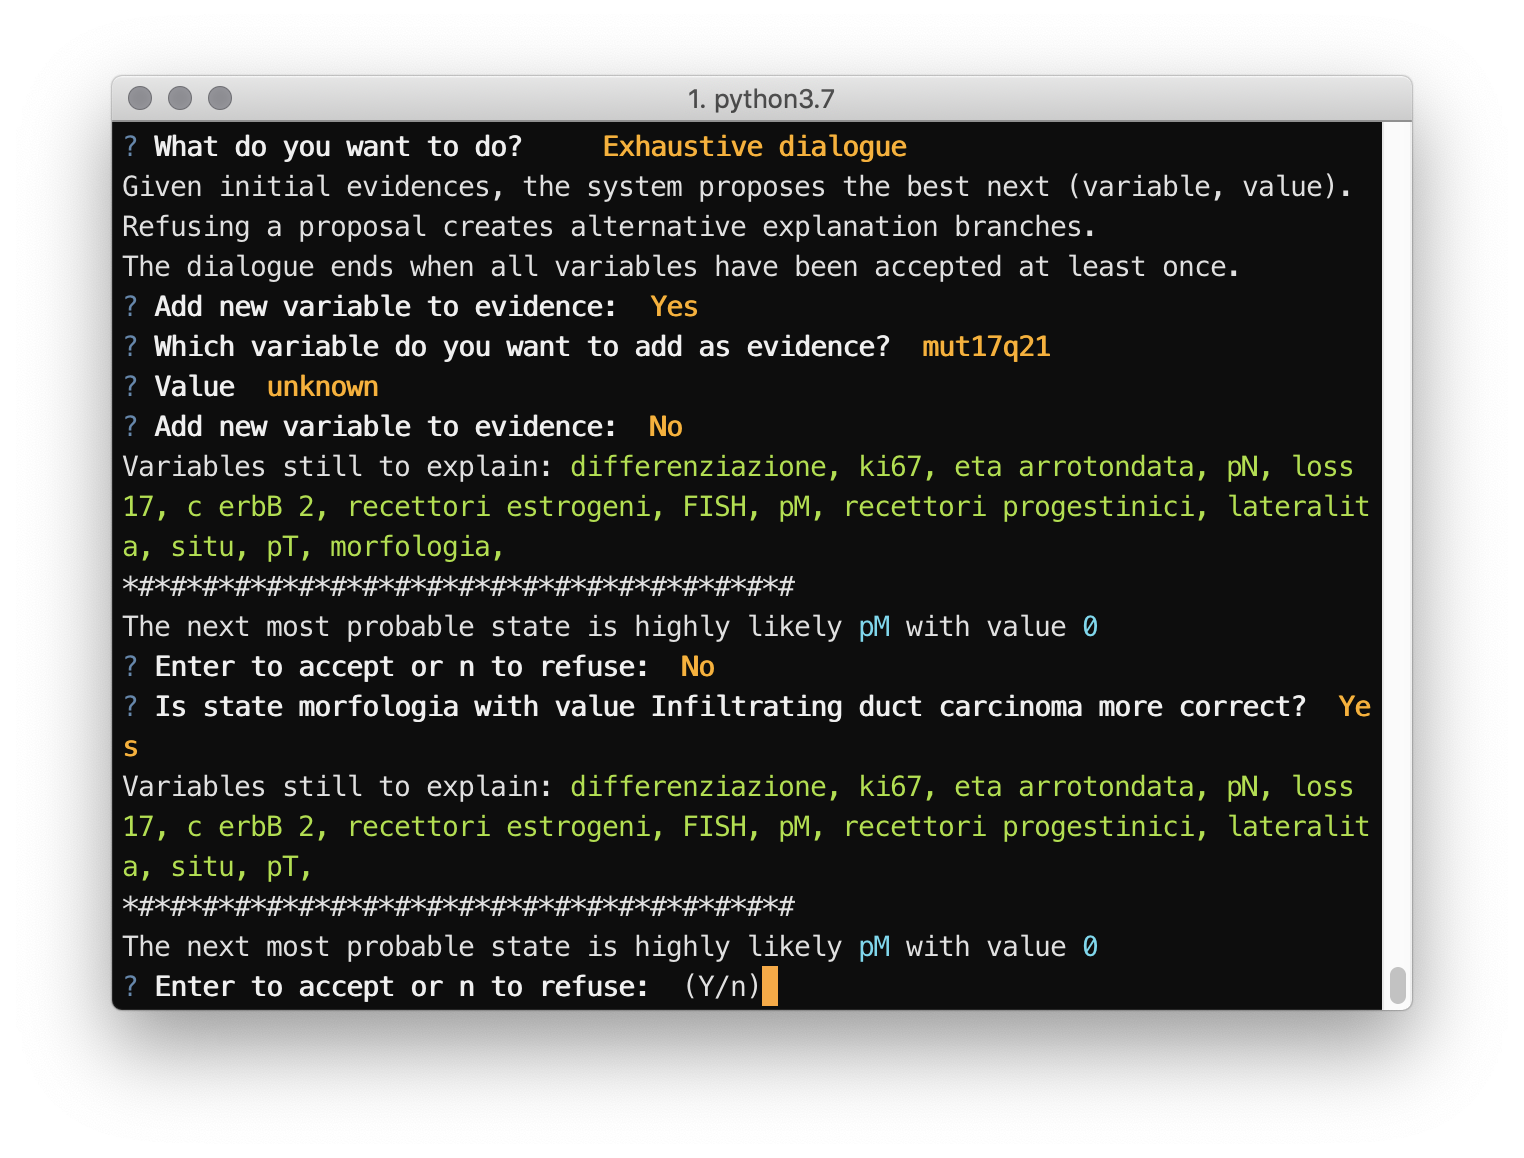
\includegraphics[width=0.7\textwidth]{methodology/images/nl-dialogue}}
\caption{Interface while executing a Dialogue}
\label{fig:nl-dialogue}
\end{figure}

\begin{figure}[htbp]
\centerline{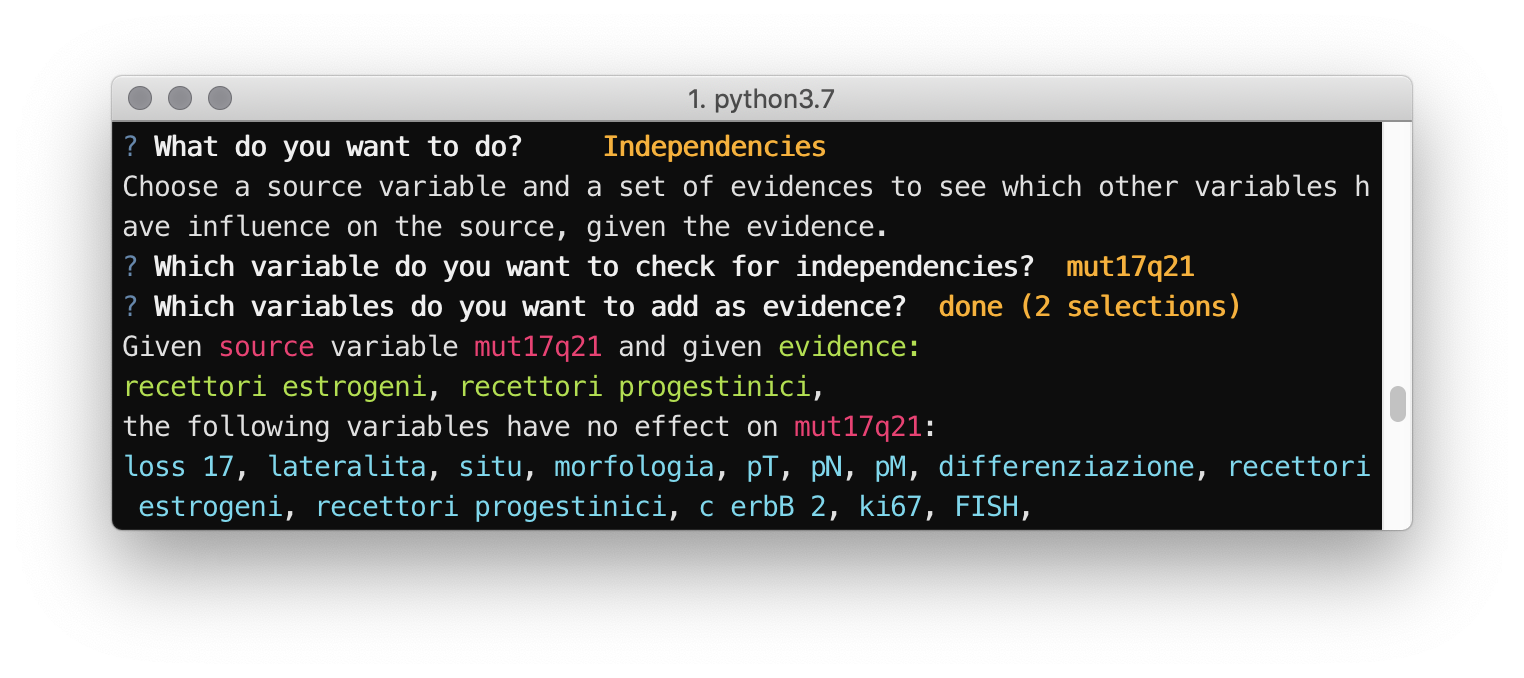
\includegraphics[width=0.7\textwidth]{methodology/images/nl-independencies-query}}
\caption{Interface while executing a query on the d-separations}
\label{fig:nl-independencies}
\end{figure}

\begin{figure}[htbp]
\centerline{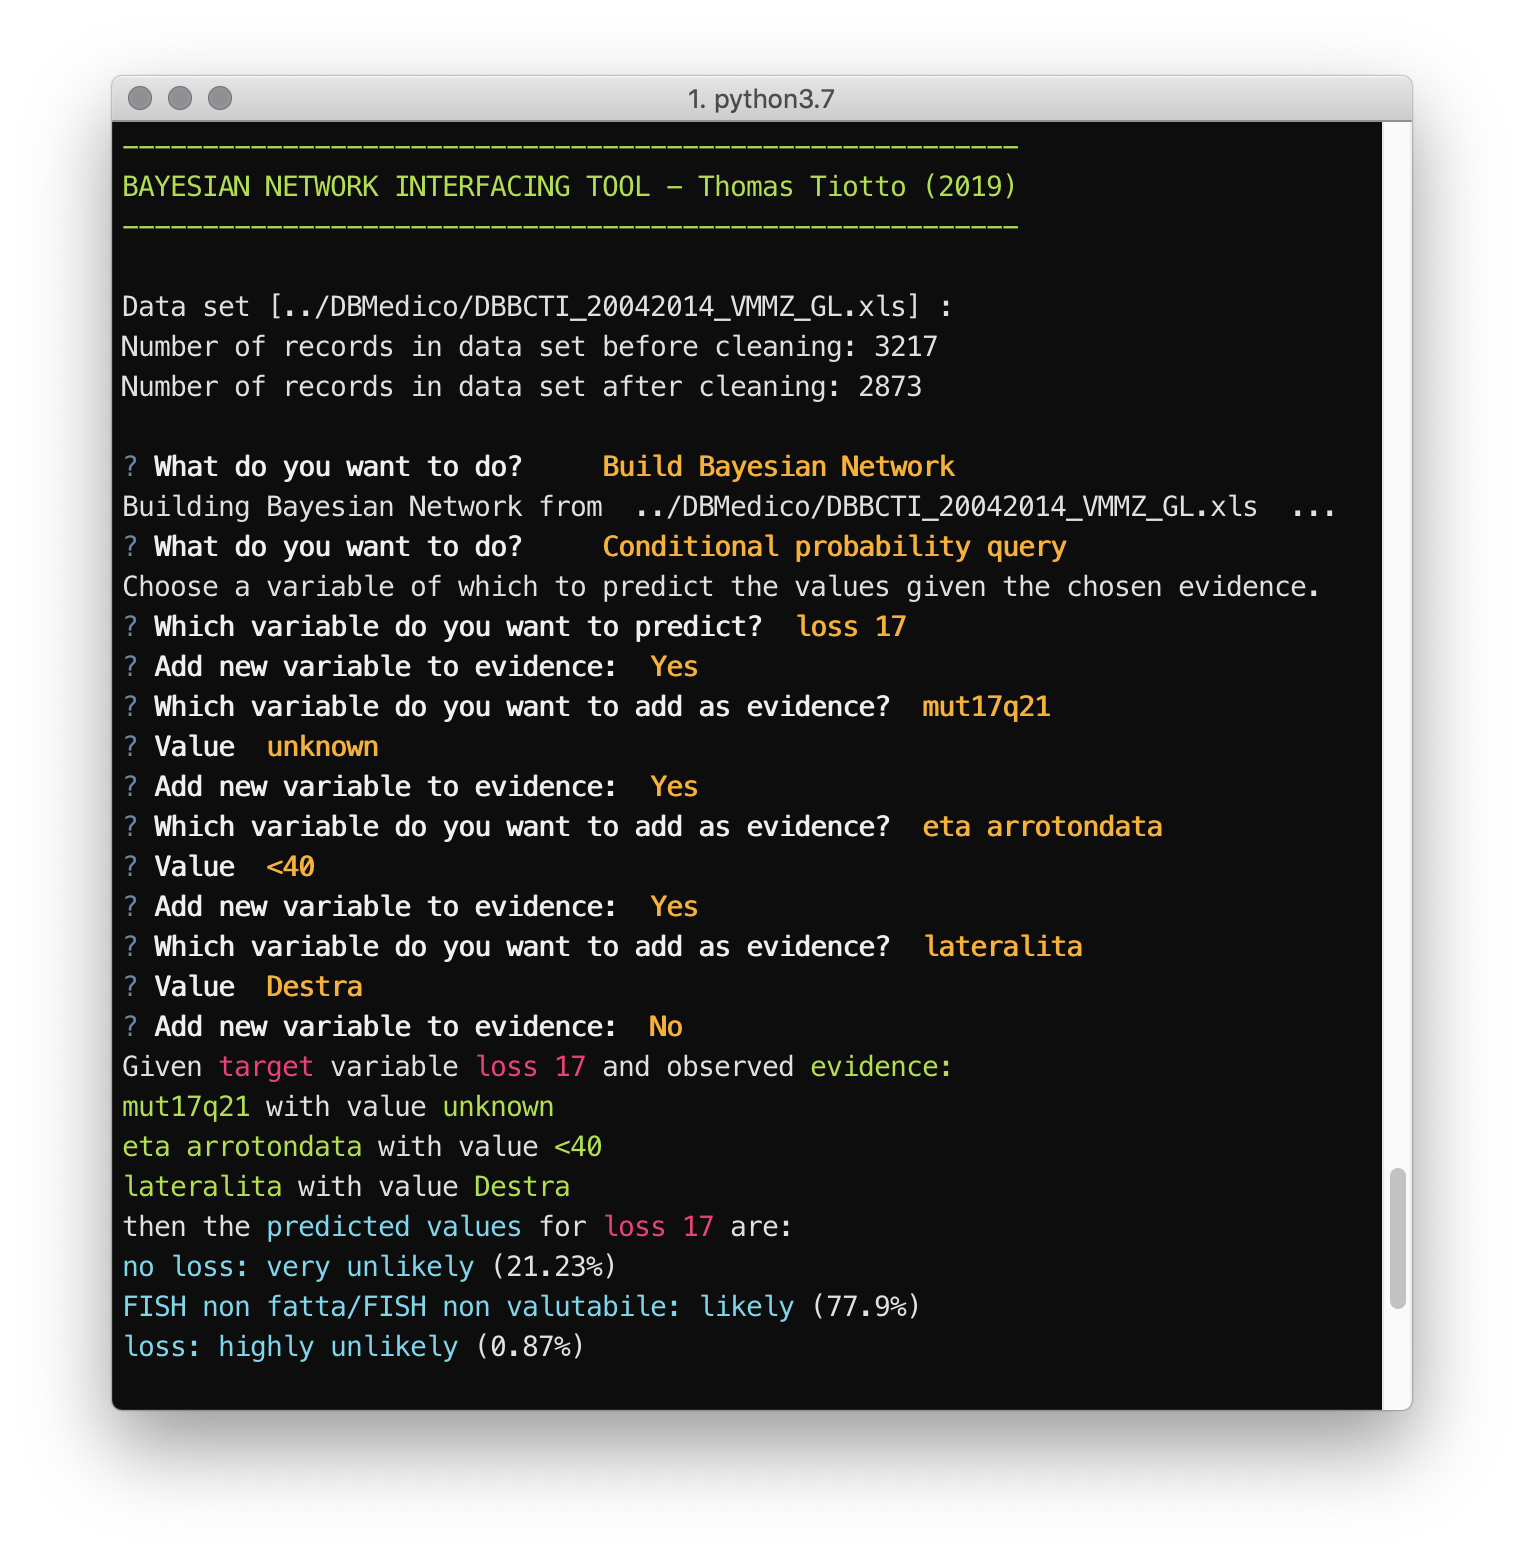
\includegraphics[width=0.7\textwidth]{methodology/images/nl-conditional-query}}
\caption{Interface while executing a conditional probability query}
\label{fig:nl-conditional}
\end{figure}

\begin{figure}[htbp]
\centerline{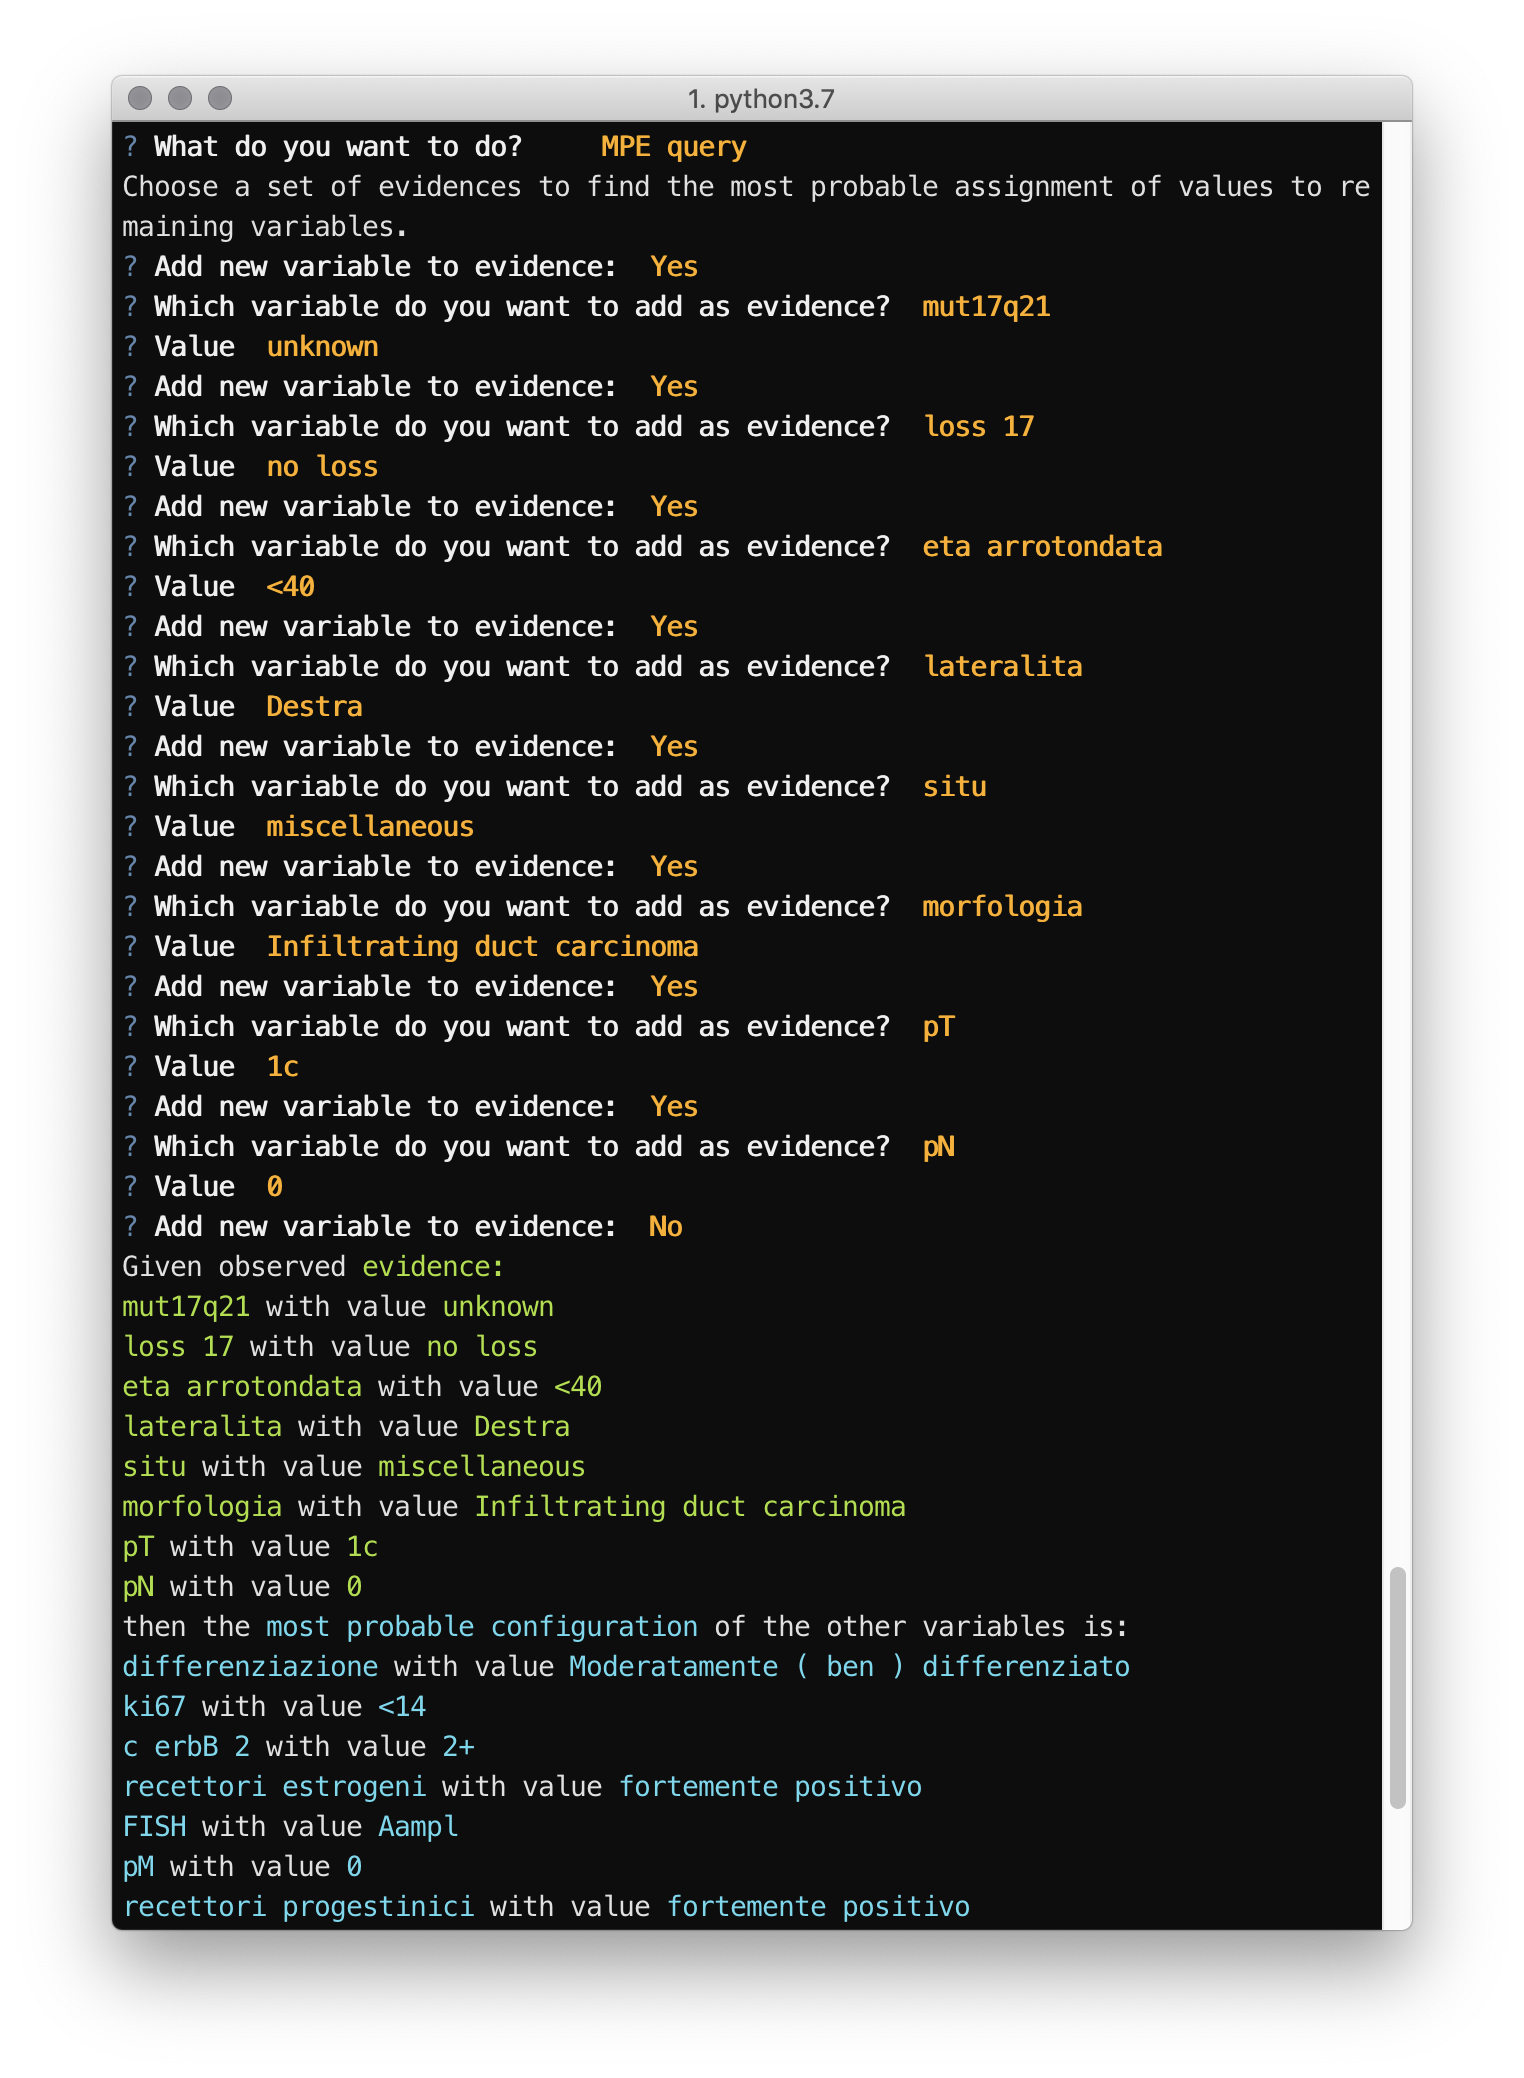
\includegraphics[width=0.7\textwidth]{methodology/images/nl-mpe-query}}
\caption{Interface while executing an MPE query}
\label{fig:nl-mpe}
\end{figure}




